\documentclass[11pt]{article}
\usepackage{times}
\newif\ifpdf
\ifx\pdfoutput\undefined
  \pdffalse
  \usepackage[dvips]{graphicx}    
  \usepackage[dvips]{color}  
\else
  \pdftrue
  \usepackage[pdftex]{graphicx}    
  \usepackage[pdftex]{color}  
\fi
\usepackage{fullpage}
\usepackage{url}
\usepackage{cite}
\usepackage{alg}
\bibliographystyle{bmc_bioinformatics}

% \draftfalse:  submission version. Figure legends & table at end. No figures included.
% \drafttrue:   online preprint. Figures and table inline.
\newif\ifdraft
\drafttrue


% Double-spacing. You can't use the doublespace.sty package; it
% conflicts with algorithm.sty.
\ifdraft
  \relax
\else
  \renewcommand{\baselinestretch}{1.5}
\fi

\def\argmax{\mathop{\mathrm{argmax}}\limits}
\def\argmin{\mathop{\mathrm{argmin}}\limits}

\setcounter{secnumdepth}{0}

\begin{document}

\title{A memory-efficient dynamic programming algorithm for optimal
alignment of a sequence to an RNA secondary structure}
\author{Sean R. Eddy\\
Howard Hughes Medical Institute \& Department of Genetics, \\
Washington University School of Medicine \\
Saint Louis, Missouri 63110 USA \\
eddy@genetics.wustl.edu}  
\date{\today}
\maketitle

\abstract{\textbf{Background:} Covariance models (CMs) are probabilistic models of RNA
secondary structure, analogous to profile hidden Markov models of
linear sequence. The dynamic programming algorithm for aligning a CM
to an RNA sequence of length $N$ is $O(N^3)$ in memory. This is only
practical for small RNAs. 

\textbf{Results:} I describe a divide and conquer variant of the
alignment algorithm that is analogous to memory-efficient Myers/Miller
dynamic programming algorithms for linear sequence alignment. The new
algorithm has an $O(N^2 \log N)$ memory complexity, at the expense of
a small constant factor in time.

\textbf{Conclusions:} Optimal ribosomal RNA structural alignments that
previously required up to 150 GB of memory now require less than 270
MB.}

\section{Background}

There are a growing number of RNA gene families and RNA motifs
\cite{Eddy01,Erdmann01}. Many (though not all) RNAs conserve a
base-paired RNA secondary structure. Computational analyses of RNA
sequence families are more powerful if they take into account both
primary sequence and secondary structure consensus
\cite{Eddy02,Dandekar95}. 

Some excellent approaches have been developed for database searching
with RNA secondary structure consensus patterns. Exact- and
approximate-match pattern searches (analogous to PROSITE patterns for
proteins) have been extended to allow patterns to specify long-range
base pairing constraints \cite{Laferriere94,Dsouza97}. In several
cases, specialized programs have been developed to recognize specific
RNA structures \cite{Dandekar95} -- for example, programs exist for
detecting transfer RNA genes
\cite{Fichant91,El-MabroukLisacek96,LoweEddy97}, group I catalytic
introns \cite{Lisacek94}, and small nucleolar RNAs
\cite{Nicoloso96,LoweEddy98}. All of these approaches, though
powerful, lack generality, and they require expert knowledge about
each particular RNA family of interest.

In primary sequence analysis, the most useful analysis techniques are
general primary sequence alignment algorithms with probabilistically
based scoring systems -- for example, the BLAST \cite{Altschul97},
FASTA \cite{Pearson88}, or CLUSTALW \cite{Thompson94b} algorithms, and
the PAM \cite{Dayhoff78} or BLOSUM \cite{Henikoff92} score
matrices. Unlike specialized programs, a general alignment algorithm
can be applied to find homologs of any query sequence(s). Unlike
pattern searches, which give yes/no answers for whether a candidate
sequence is a match, a scoring system gives a meaningful score that
allows ranking candidate hits by their statistical significance. It is
of interest to develop general alignment algorithms for RNA secondary
structures.

The problem I consider here is as follows.  I am given a multiple
alignment of an RNA sequence family for which I know the consensus
secondary structure. I want to search a sequence database for homologs
that significantly match the sequence \emph{and structure} of my
query. The sequence analysis analogue is the use of profile hidden
Markov models (profile HMMs) to model multiple alignments of conserved
protein domains, and to discover new homologues in sequence databases
\cite{Krogh94,Eddy98}. For instance, if we had an RNA structure
equivalent of the HMMER profile HMM program suite
(\url{http://hmmer.wustl.edu/}) it would be possible to develop and
efficiently maintain databases of conserved RNA structures and
multiple alignments, analogous to the Pfam or SMART databases of
conserved protein domains \cite{Bateman02,LetunikBork02}.

Stochastic context free grammar (SCFG) algorithms provide a general
approach to RNA structure alignment
\cite{Eddy94,Sakakibara94c,Durbin98}. SCFGs allow the strong pairwise
residue correlations in non-pseudoknotted RNA secondary structure to
be taken into account in RNA alignments. SCFGs can be aligned to
sequences using a dynamic programming algorithm that guarantees
finding a mathematically optimal solution in polynomial time. SCFG
alignment algorithms can be thought of as an extension of sequence
alignment algorithms (particularly those with fully probabilistic,
hidden Markov model formulations) into an additional dimension
necessary to deal with 2D RNA secondary structure.

While SCFGs provide a natural mathematical framework for RNA secondary
structure alignment problems, SCFG algorithms have high computational
complexity that has impeded their practical application. Optimal
SCFG-based structural alignment of an RNA structure to a sequence
costs $O(N^3)$ memory and $O(N^4)$ time for a sequence of length $N$,
compared to $O(N^2)$ memory and time for sequence alignment
algorithms. (Corpet and Michot described a program that implements a
different general dynamic programming algorithm for RNA alignment;
their algorithm solves the same problem but even less efficiently,
requiring $O(N^4)$ memory and $O(N^5)$ time \cite{Corpet94}.)
SCFG-based alignments of small structural RNAs are feasible. Using my
COVE software
(\url{http://www.genetics.wustl.edu/eddy/software#cove}), transfer RNA
alignments ($\sim 75$ nucleotides) take about 0.2 cpu second and 3 Mb
of memory. Most genome centers now use an COVE-based search program,
tRNAscan-SE, for annotating transfer RNA genes
\cite{LoweEddy97}. However, many larger RNAs of interest are outside
the capabilities of the standard SCFG alignment algorithm. Alignment
of a small subunit (SSU) ribosomal RNA sequence to the SSU rRNA
consensus structure would take about 23 GB of RAM and an hour of CPU
time. The steep memory requirement constitutes a significant barrier
to the practicality of SCFG algorithms.

Notredame \emph{et al.} pointed specifically to this problem
\cite{Notredame97}.  They described RAGA, a program that uses a
genetic algorithm (GA) to optimize a pairwise RNA alignment using an
objective function that includes base pairing terms. Because GAs have
an $O(N)$ memory requirement, RAGA can find reasonable solutions for
large RNA alignment problems, including ribosomal RNA alignments. A
different memory-efficient approach has also been described
\cite{Lenhof98,LenhofVingron98}. However, both approaches are
approximate and cannot guarantee a mathematically optimal solution, in
contrast to the (mathematically) optimal but more expensive dynamic
programming approaches.

Here, I introduce a dynamic programming solution to the problem of
structural alignment of large RNAs. The central idea is a divide and
conquer strategy. For linear sequence alignment, a divide and conquer
algorithm was introduced by Hirschberg \cite{Hirschberg75}, an
algorithm known in the computational biology community as the
Myers/Miller algorithm \cite{MyM-88a}. (Ironically, at the time,
dynamic programming methods for optimal sequence alignment were well
known, but were considered impractical on 1970's era computers because
of the ``extreme'' $O(N^2)$ memory requirement.) Myers/Miller reduces
the memory complexity of a dynamic programming sequence alignment
algorithm from $O(N^2)$ to $O(N)$, at the cost of a roughly two-fold
increase in CPU time. Here I show that a divide and conquer strategy
can also be applied to the RNA structural alignment problem, greatly
reducing the memory requirement of SCFG alignments and making optimal
structural alignment of large RNAs possible.

I will strictly be dealing with the problem of aligning a target
sequence of unknown secondary structure to a query of known RNA
structure. By ``secondary structure'' I mean nested (nonpseudoknotted)
pairwise RNA secondary structure interactions, primarily Watson-Crick
base pairs but also permitting noncanonical base pairs. This RNA
structural alignment problem is different from the problem of aligning
two known RNA secondary structures together \cite{Shapiro90}, and from
the problem of aligning two RNA sequences of unknown structure
together under a secondary structure-aware scoring system
\cite{Sankoff85,Gorodkin01,MathewsTurner02}.

\section{Algorithm}

\subsection{Prelude: the simpler case of sequence alignment}

The essential concepts of a divide and conquer alignment algorithm are
most easily understood for the case of linear sequence alignment
\cite{Hirschberg75,MyM-88a}.

Dynamic programming (DP) algorithms for sequence alignment fill in an
$N \times M$ DP matrix of scores $F(i,j)$ for two sequences of lengths
$N$ and $M$ ($N < M$)  \cite{Needleman70,Smith81}. Each score
$F(i,j)$ is the score of the optimal alignment of prefix $x_1..x_i$ of
one sequence to prefix $y_1..y_j$ of the other. These scores are
calculated iteratively, e.g.  for global (Needleman/Wunsch) alignment:

\[  F(i,j) = \max \left\{ \begin{array}{l}
                       F(i-1,j-1) + \mbox{score for aligning $x_i, y_j$} \\
                       F(i-1,j) - \mbox{cost of a gap character} \\
                       F(i,j-1) - \mbox{cost of a gap character} \\
                       \end{array} \right. \]

At the end, $F(N,M)$ contains the score of the optimal alignment. The
alignment itself is recovered by tracing the individual optimal steps
backwards through the matrix, starting from cell $(N,M)$. The
algorithm is $O(NM)$ in both time and memory.

If we are only interested in the score, not the alignment itself, the
whole $F$ matrix does not have to be kept in memory. The iterative
calculation only depends on the current and previous row of the
matrix. Keeping two rows in memory suffices (in fact, a compulsively
efficient implementation can get away with $N+1$ cells). A score-only
calculation can be done in $O(N)$ space.

The fill stage of DP alignment algorithms may be run either forwards
and backwards. We can just as easily calculate the optimal score
$B(i,j)$ of the best alignment of the \emph{suffix} $i+1..N$ of
sequence 1 to the suffix $j+1..M$ of sequence 2, until one obtains
$B(0,0)$, the overall optimal score -- the same number as $F(N,M)$.

The sum of $F(i,j)$ and $B(i,j)$ at any cell in the optimal path
through the DP matrix is also the optimal overall alignment score.
More generally, $F(i,j) + B(i,j)$ at any cell $(i,j)$ is the score of
the best alignment that uses that cell. Therefore, since we know the
optimal alignment must pass through any given row $i$
\emph{somewhere}, we can pick some row $i$ in the middle of sequence
$x$, run the forward calculation to $i$ to obtain row $F(i)$, run the
backwards calculation back to $i$ to get row $B(i)$, and then find
$\argmax\nolimits_j F(i,j) + B(i,j)$. Now I know the optimal alignment
passes through cell $(i,j)$. (For clarity, I am leaving out details of
how indels and local alignments are handled.)

This divides the alignment into two smaller alignment problems, and
these smaller problems can themselves be subdivided by the same trick.
Thus, the complete optimal alignment can be found by a recursive
series of split point calculations. Although this seems laborious --
each calculation is giving us only a single point in the alignment --
if we choose our split row $i$ to be in the middle, the size of the
two smaller DP problems is decreased by about 4-fold at each split. A
complete alignment thus costs only about $1 + \frac{2}{4} +
\frac{4}{16} + \ldots \simeq 2$ times as much CPU time as doing the
alignment in a single DP matrix calculation, but the algorithm is
$O(N)$ in memory.

A standard dynamic programming alignment algorithm for SCFGs is the
Cocke-Younger-Kasami (CYK) algorithm, which finds an optimal parse
tree (e.g. alignment) for a model and a sequence
\cite{Kasami65,Younger67,HopcroftUllman79,Durbin98}.\footnote{CYK is
usually described in the literature as a dynamic programming
recognition algorithm for nonstochastic CFGs in Chomsky normal form,
rather than as a dynamic programming parsing algorithm for SCFGs in
any form. The use of the name ``CYK'' here is therefore a little imprecise
\cite{Durbin98}.}  CYK can be run in a memory-saving ``score only''
mode. The DP matrix for CYK can also be filled in two opposite
directions - either ``inside'' or ``outside'', analogous to forward
and backward DP matrix fills for linear sequence alignment.  I will
refer to these algorithms as CYK/inside and CYK/outside (or just
\texttt{inside} and \texttt{outside}), but readers familiar with SCFG
algorithms should not confuse them with the SCFG Inside and Outside
algorithms \cite{Lari90,Lari91} which sum over all possible parse
trees rather than finding one optimal parse tree. I am always talking
about the CYK algorithm in this paper, and by ``inside'' and
``outside'' I am only referring generically to the direction of the
CYK DP calculation.

The CYK/inside and CYK/outside algorithms are not as nicely
symmetrical as the forward and backward DP fills are in sequence
alignment algorithms. The splitting procedure that one obtains does
not generate identical types of subproblems, so the divide and conquer
procedure for SCFG-based RNA alignment is not as obvious.

\subsection{Definition and construction of a covariance model}

The divide and conquer algorithm I will describe is specific for RNA
``covariance models'' (CMs). A covariance model is a profile
stochastic context free grammar designed to model a consensus RNA
secondary structure with position-specific scores
\cite{Eddy94,Durbin98}. My algorithm takes advantage of features of
CMs that do not apply to SCFGs in general.  Therefore I start with an
introduction to what CMs are, how they correspond to a known RNA
secondary structure, and how they are built and parameterized.

\subsubsection{Definition of a stochastic context free grammar}

A stochastic context free grammar (SCFG) consists of the following:

\begin{itemize}
\item $M$ different nonterminals (here called \emph{states}). I will use capital
      letters to refer to specific nonterminals; $V$ and $Y$ will be used
      to refer generically to unspecified nonterminals.
\item $K$ different terminal symbols (e.g. the observable alphabet,
      {a,c,g,u} for RNA). I will use small letters $a,b$ to refer
      generically to terminal symbols.
\item a number of \emph{production rules} of the form: $V \rightarrow
\gamma$, where $\gamma$ can be any string of nonterminal and/or
terminal symbols, including (as a special case) the empty string
$\epsilon$.\footnote{$\epsilon$ productions are ``shrinking'' rules,
in which the right hand side of the production is shorter than the
left. These are technically not allowed in CFGs. This restriction is
important in proofs of the properties of CFGs. A CFG with $\epsilon$
productions can always be converted to an equivalent, formally correct
CFG without $\epsilon$ productions; for example, two rules $V
\rightarrow a V b; V \rightarrow \epsilon$ are equivalent to $V
\rightarrow a V b; V \rightarrow ab$. $\epsilon$ productions are no
problem in dynamic programming alignment, and indeed are more
convenient, because they reduce redundancy and simplify initialization
of dynamic programming parsing algorithms.}
\item Each production rule is associated with a probability, such that
      the sum of the production probabilities for any given
      nonterminal $V$ is equal to 1.
\end{itemize} 

\subsubsection{SCFG productions allowed in covariance models}

A covariance model is a specific repetitive ``profile SCFG''
architecture consisting of groups of model states that are associated
with base pairs and single-stranded positions in an RNA secondary
structure consensus. A covariance model has seven types of states and
production rules:

\vspace{0.5em}
\begin{tabular}{lllll}
State type & Description             &  Production             & Emission & Transition\\ \hline
P & (pair emitting)   & $P \rightarrow a Y b$ & $e(a,b)$ & $t(Y)$  \\
L & (left emitting)   & $L \rightarrow a Y$   & $e(a)$   & $t(Y)$  \\
R & (right emitting)  & $R \rightarrow Y a$   & $e(a)$   & $t(Y)$  \\
B & (bifurcation)     & $B \rightarrow S S$   & 1     &     1     \\
D & (delete)          & $D \rightarrow Y$     & 1     &   $t(Y)$  \\
S & (start)           & $S \rightarrow Y$     &    1     & $t(Y)$  \\
E & (end)             & $E \rightarrow \epsilon$ & 1     &     1     \\
\end{tabular}
\vspace{0.5em}

Each overall production probability is the independent product of an
emission probability $e$ and a transition probability $t$ (analogous
to hidden Markov models). For example, a pair state $P$ produces two
correlated letters $a$ and $b$ (e.g. one of 16 possible base pairs)
with probability $e(a,b)$ and transits to one of several possible new
states $Y$ of various types with probability $t(Y)$.  A bifurcation
(B) state splits into two new start ($S$) states with probability 1.
The E state is a special case $\epsilon$ production that terminates a
derivation.

A CM consists of many states of these seven basic types, each with its
own emission and transition probability distributions, and its own set
of states that it can transition to. Consensus base pairs will be
modeled by P states, consensus single stranded residues by L and
R states, insertions relative to the consensus by more L and R
states, deletions relative to consensus by D states, and the
branching topology of the RNA secondary structure by B, S, and E
states. The procedure for starting from an input multiple alignment
and determining how many states, what types of states, and how they
are interconnected by transition probabilities is described next.

\subsubsection{From consensus structural alignment to guide tree}

Figure~\ref{fig:input_alignment} shows an example input file: a
multiple sequence alignment of homologous RNAs, with a line describing
the consensus RNA secondary structure. The first step of building a CM
is to produce a binary \emph{guide tree} of \emph{nodes} representing
the consensus secondary structure. The guide tree is a parse tree for
the consensus structure, with nodes as nonterminals and alignment
columns as terminals.

\ifdraft
\begin{figure}[t]
\begin{center}
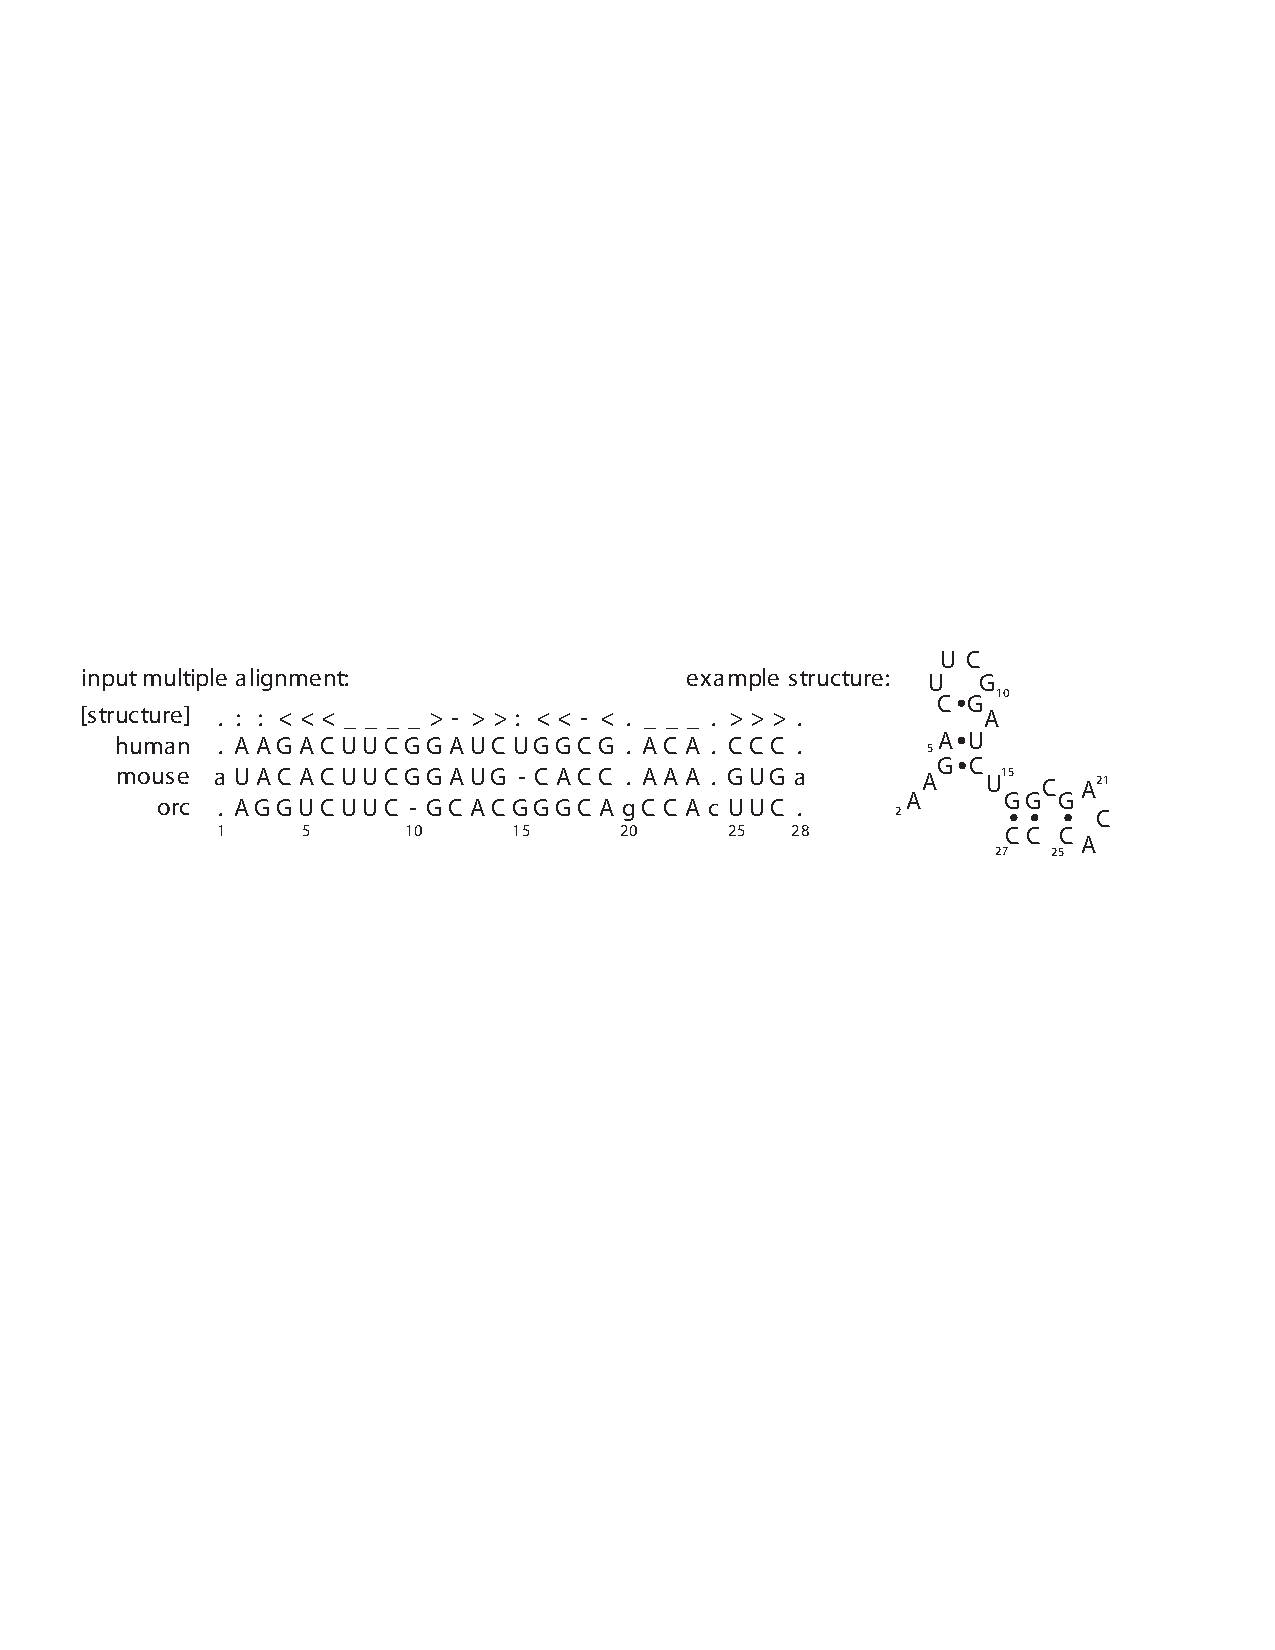
\includegraphics[width=5in]{Figures/input_alignment}
\end{center}
\caption{\textbf{An example RNA sequence family.} Top: a toy multiple
alignment of three sequences, with 28 total columns, 24 of which will
be modeled as consensus positions. The [structure] line annotates the
consensus secondary structure: $>$ and $<$ symbols mark base pairs,
x's mark consensus single stranded positions, and .'s mark
``insert'' columns that will not be considered part of the consensus
model. Bottom: the secondary structure of the ``human'' sequence.} 
\label{fig:input_alignment}
\end{figure}
\fi

The guide tree has eight types of nodes:

\vspace{0.5em}
\begin{tabular}{lll}
Node      & Description        &  Main state type          \\ \hline
MATP  & (pair)                 & P \\
MATL  & (single strand, left)  & L \\
MATR  & (single strand, right) & R \\
BIF   & (bifurcation)          & B \\
ROOT  & (root)                 & S \\
BEGL  & (begin, left)          & S \\
BEGR  & (begin, right)         & S \\
END   & (end)                  & E \\
\end{tabular}
\vspace{0.5em}
 
These consensus node types correspond closely with a CM's final state
types. Each node will eventually contain one or more states. The guide
tree deals with the consensus structure. For individual sequences, we
will need to deal with insertions and deletions with respect to this
consensus. The guide tree is the skeleton on which we will organize
the CM. For example, a MATP node will contain a P-type state to
model a consensus base pair; but it will also contain several other
states to model infrequent insertions and deletions at or adjacent to
this pair.

The input alignment is first used to construct a consensus secondary
structure (Figure~\ref{fig:cm_nodetree}) that defines which aligned
columns will be ignored as non-consensus (and later modeled as
insertions relative to the consensus), and which consensus alignment
columns are base-paired to each other. Here I assume that both the
structural annotation and the labeling of insert versus consensus
columns is given in the input file, as shown in the line marked
``[structure]'' in the alignment in Figure~\ref{fig:input_alignment}.
Alternatively, automatic methods might be employed. A consensus
structure could be predicted from comparative analysis of the
alignment \cite{Chiu91,Gutell92,Eddy94}.  The consensus columns could
be chosen as those columns with less than a certain fraction of gap
symbols, or by a maximum likelihood criterion, as is done for profile
HMM construction \cite{Krogh94,Durbin98}.

\ifdraft
\begin{figure}[t]
\begin{center}
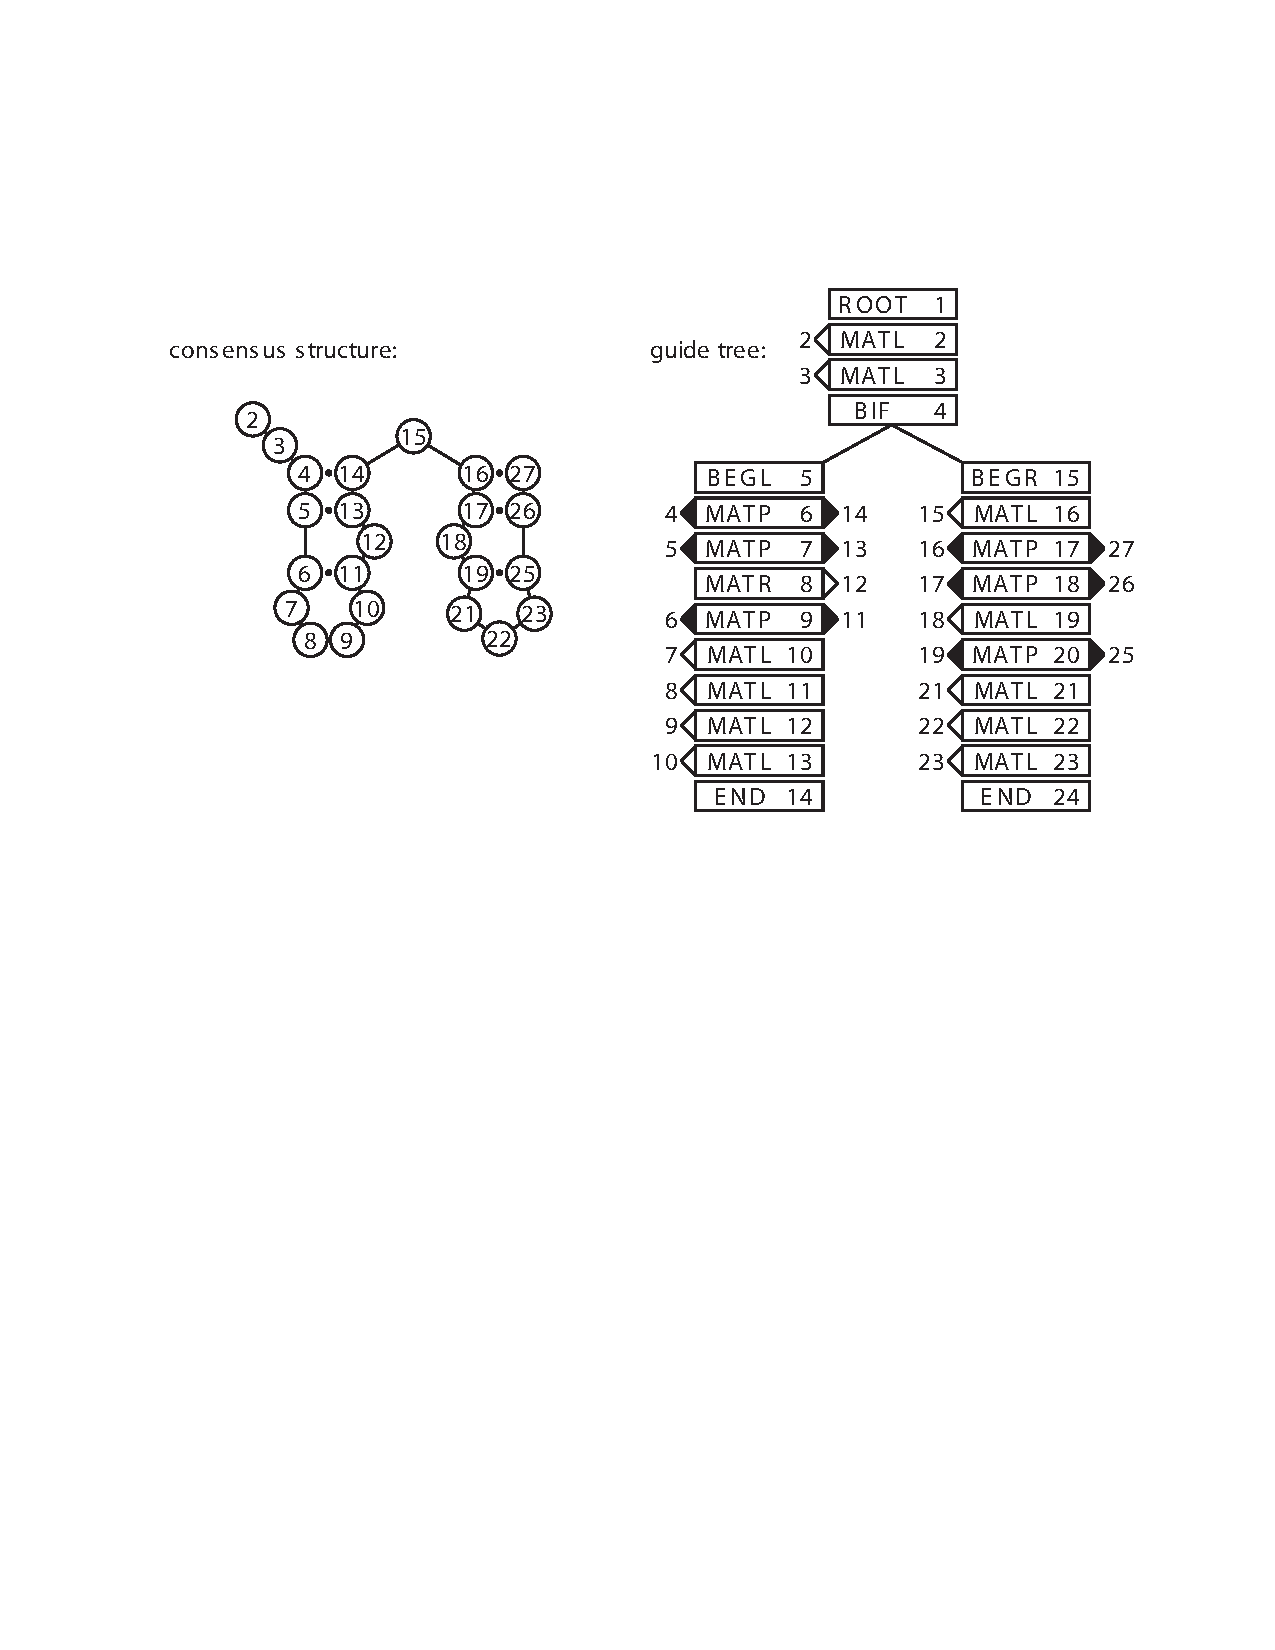
\includegraphics[width=5in]{Figures/cm_nodetree}
\end{center}
\caption{\textbf{The structural alignment is converted to a guide
tree.} Left: the consensus secondary structure is derived from the
annotated alignment in Figure~\ref{fig:input_alignment}. Numbers in
the circles indicate alignment column coordinates: e.g.  column 4 base
pairs with column 14, and so on. Right: the CM guide tree
corresponding to this consensus structure. The nodes of the tree are
numbered 1..24 in preorder traversal (see text). MATP, MATL, and MATR
nodes are associated with the columns they generate: e.g., node 6 is a
MATP (pair) node that is associated with the base-paired columns 4 and
14.}
\label{fig:cm_nodetree}
\end{figure}
\fi

Given the consensus structure, consensus base pairs are assigned to
MATP nodes and consensus unpaired columns are assigned to MATL or MATR
nodes. One ROOT node is used at the head of the tree.  Multifurcation
loops and/or multiple stems are dealt with by assigning one or more
BIF nodes that branch to subtrees starting with BEGL or BEGR head
nodes. (ROOT, BEGL, and BEGR start nodes are labeled differently
because they will be expanded to different groups of states; this has
to do with avoiding ambiguous parse trees for individual sequences, as
described below.) Alignment columns that are considered to be
insertions relative to the consensus structure are ignored at this
stage.

In general there will be more than one possible guide tree for any
given consensus structure. Almost all of this ambiguity is eliminated
by three conventions: (1) MATL nodes are always used instead of MATR
nodes where possible, for instance in hairpin loops; (2) in describing
interior loops, MATL nodes are used before MATR nodes; and (3) BIF
nodes are only invoked where necessary to explain branching secondary
structure stems (as opposed to unnecessarily bifurcating in single
stranded sequence). One source of ambiguity remains. In invoking a
bifurcation to explain alignment columns $i..j$ by two substructures
on columns $i..k$ and $k+1..j$, there will be more than one possible
choice of $k$ if $i..j$ is a multifurcation loop containing three or
more stems. The choice of $k$ impacts the performance of the divide
and conquer algorithm; for optimal time performance, we will want
bifurcations to split into roughly equal sized alignment problems, so
I choose the $k$ that makes $i..k$ and $k+1..j$ as close to the same
length as possible.

The result of this procedure is the guide tree. The nodes of the guide
tree are numbered in preorder traversal (e.g. a recursion of ``number
the current node, visit its left child, visit its right child'': thus
parent nodes always have lower indices than their children). The guide
tree corresponding to the input multiple alignment in
Figure~\ref{fig:input_alignment} is shown in
Figure~\ref{fig:cm_nodetree}.

\subsubsection{From guide tree to covariance model}

A CM must deal with insertions and deletions in individual sequences
relative to the consensus structure. For example, for a consensus base
pair, either partner may be deleted leaving a single unpaired residue,
or the pair may be entirely deleted; additionally, there may be
inserted nonconsensus residues between this pair and the next pair in
the stem. Accordingly, each node in the master tree is expanded into
one or more \emph{states} in the CM as follows:

\vspace{0.5em}
\begin{tabular}{llccc}
       &                     & total \#& \# of split& \# of insert\\
Node   &  States             & states  & states     & states \\ \hline
MATP   & [MP ML MR D] IL IR  &   6     &   4        &  2   \\
MATL   & [ML D] IL           &   3     &   2    &  1   \\
MATR   & [MR D] IR           &   3     &   2    &  1   \\
BIF    & [B]                 &   1     &   1    &  0   \\
ROOT   & [S] IL IR           &   3     &   1    &  2   \\
BEGL   & [S]                 &   1     &   1    &  0   \\
BEGR   & [S] IL              &   2     &   1    &  1   \\
END    & [E]                 &   1     &   1    &  0   \\ \hline
\end{tabular}
\vspace{0.5em}

Here we distinguish between consensus (``M'', for ``match'') states
and insert (``I'') states. ML and IL, for example, are both L type
states with L type productions, but they will have slightly different
properties, as described below.

The states are grouped into a \emph{split set} of 1-4 states (shown in
brackets above) and an \emph{insert set} of 0-2 insert states. The
split set includes the main consensus state, which by convention is
first. One and only one of the states in the split set must be visited
in every parse tree (and this fact will be exploited by the divide and
conquer algorithm). The insert state(s) are not obligately visited,
and they have self-transitions, so they will be visited zero or more
times in any given parse tree.

State transitions are then assigned as follows. For bifurcation nodes,
the B state makes obligate transitions to the S states of the child
BEGL and BEGR nodes. For other nodes, each state in a split set has a
possible transition to every insert state in the \emph{same} node, and
to every state in the split set of the \emph{next} node. An IL state
makes a transition to itself, to the IR state in the same node (if
present), and to every state in the split set of the next node. An IR
state makes a transition to itself and to every state in the split set
of the next node.

This arrangement of transitions guarantees that (given the guide tree)
there is unambiguously one and only one parse tree for any given
individual structure. This is important. The algorithm will find a
maximum likelihood parse tree for a given sequence, and we wish to
interpret this result as a maximum likelihood structure, so there must
be a one to one relationship between parse trees and secondary
structures \cite{Giegerich00}.

The final CM is an array of $M$ states, connected as a directed graph
by transitions $t_v(y)$ (or probability 1 transitions $v \rightarrow
(y,z)$ for bifurcations) with the states numbered such that $(y,z)
\geq v$. There are no cycles in the directed graph other than cycles
of zero length (e.g. the self-transitions of the insert states). We
can think of the CM as an array of states in which all transition
dependencies run in one direction; we can do an iterative dynamic
programming calculation through the model states starting with the
last numbered end state $M$ and ending in the root state $1$.  An
example CM, corresponding to the input alignment of
Figure~\ref{fig:input_alignment}, is shown in
Figure~\ref{fig:cm_graph}.

As a convenient side effect of the construction procedure, it is
guaranteed that the transitions from any state are to a
\emph{contiguous} set of child states, so the transitions for state
$v$ may be kept as an offset and a count. For example, in
Figure~\ref{fig:cm_graph}, state 12 (an MP) connects to states 16, 17,
18, 19, 20, and 21. We can store this as an offset of 4 to the first
connected state, and a total count of 6 connected states.  We know
that the offset is the distance to the next non-split state in the
current node; we also know that the count is equal to the number of
insert states in the current node, plus the number of split set states
in the next node. These properties make establishing the connectivity
of the CM trivial. Similarly, all the parents of any given state are
also contiguously numbered, and can be determined analogously. We are
also guaranteed that the states in a split set are numbered
contiguously.  This contiguity is exploited by the divide and conquer
implementation.

\ifdraft
\begin{figure}[tp]
\begin{center}
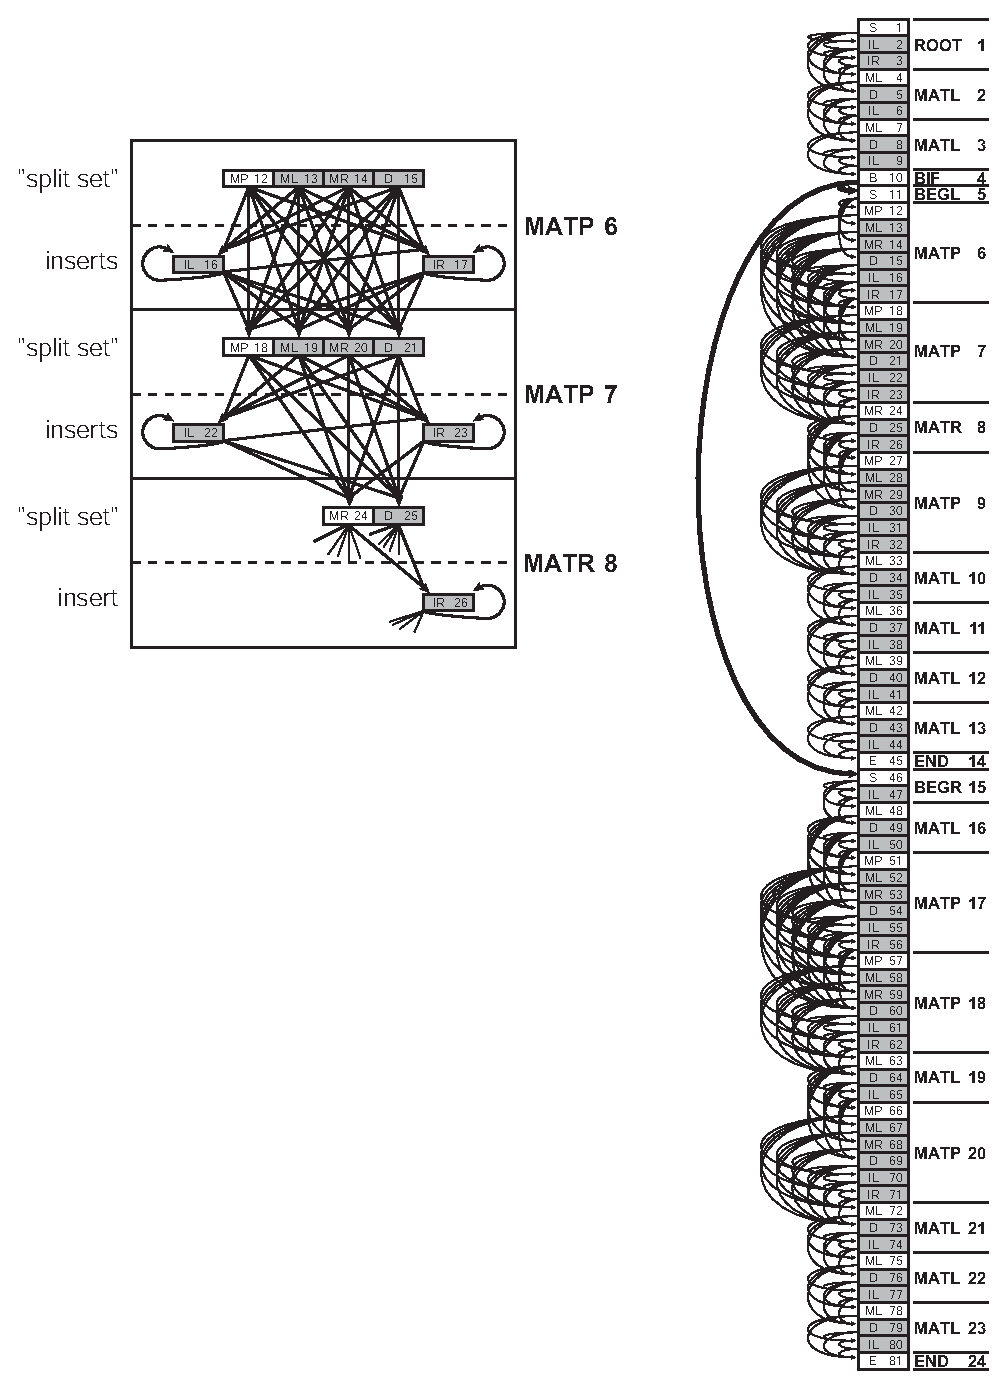
\includegraphics[width=5in]{Figures/cm_graph}
\end{center}
\caption{\textbf{A complete covariance model.} Right: the CM
corresponding to the alignment in Figure~\ref{fig:input_alignment}.
The model has 81 states (boxes, stacked in a vertical array). Each
state is associated with one of the 24 nodes of the guide tree (text
to the right of the state array). States corresponding to the
consensus are in white. States responsible for insertions and
deletions are gray. The transitions from bifurcation state B10 to
start states S11 and S46 are in bold because they are special: they
are an obligate (probability 1) bifurcation. All other transitions
(thin arrows) are associated with transition probabilities.  Emission
probability distributions are not represented in the figure. Left: the
states are also arranged according to the guide tree. A blow up of
part of the model corresponding to nodes 6, 7, and 8 shows
more clearly the logic of the connectivity of transition probabilities
(see main text), and also shows why any parse tree must transit through
one and only one state in each ``split set''.}
\label{fig:cm_graph}
\end{figure}
\fi

\subsubsection{Parameterization}

Using the guide tree and the final CM, each individual sequence in the
input multiple alignment can be converted unambiguously to a CM parse
tree, as shown in Figure~\ref{fig:parsetrees}. Counts for observed
state transitions and singlet/pair emissions are then collected from
these parse trees. The observed counts are converted to transition and
emission probabilities by standard procedures. I calculate maximum a
posteriori parameters, using Dirichlet priors.

\ifdraft
\begin{figure}[t]
\begin{center}
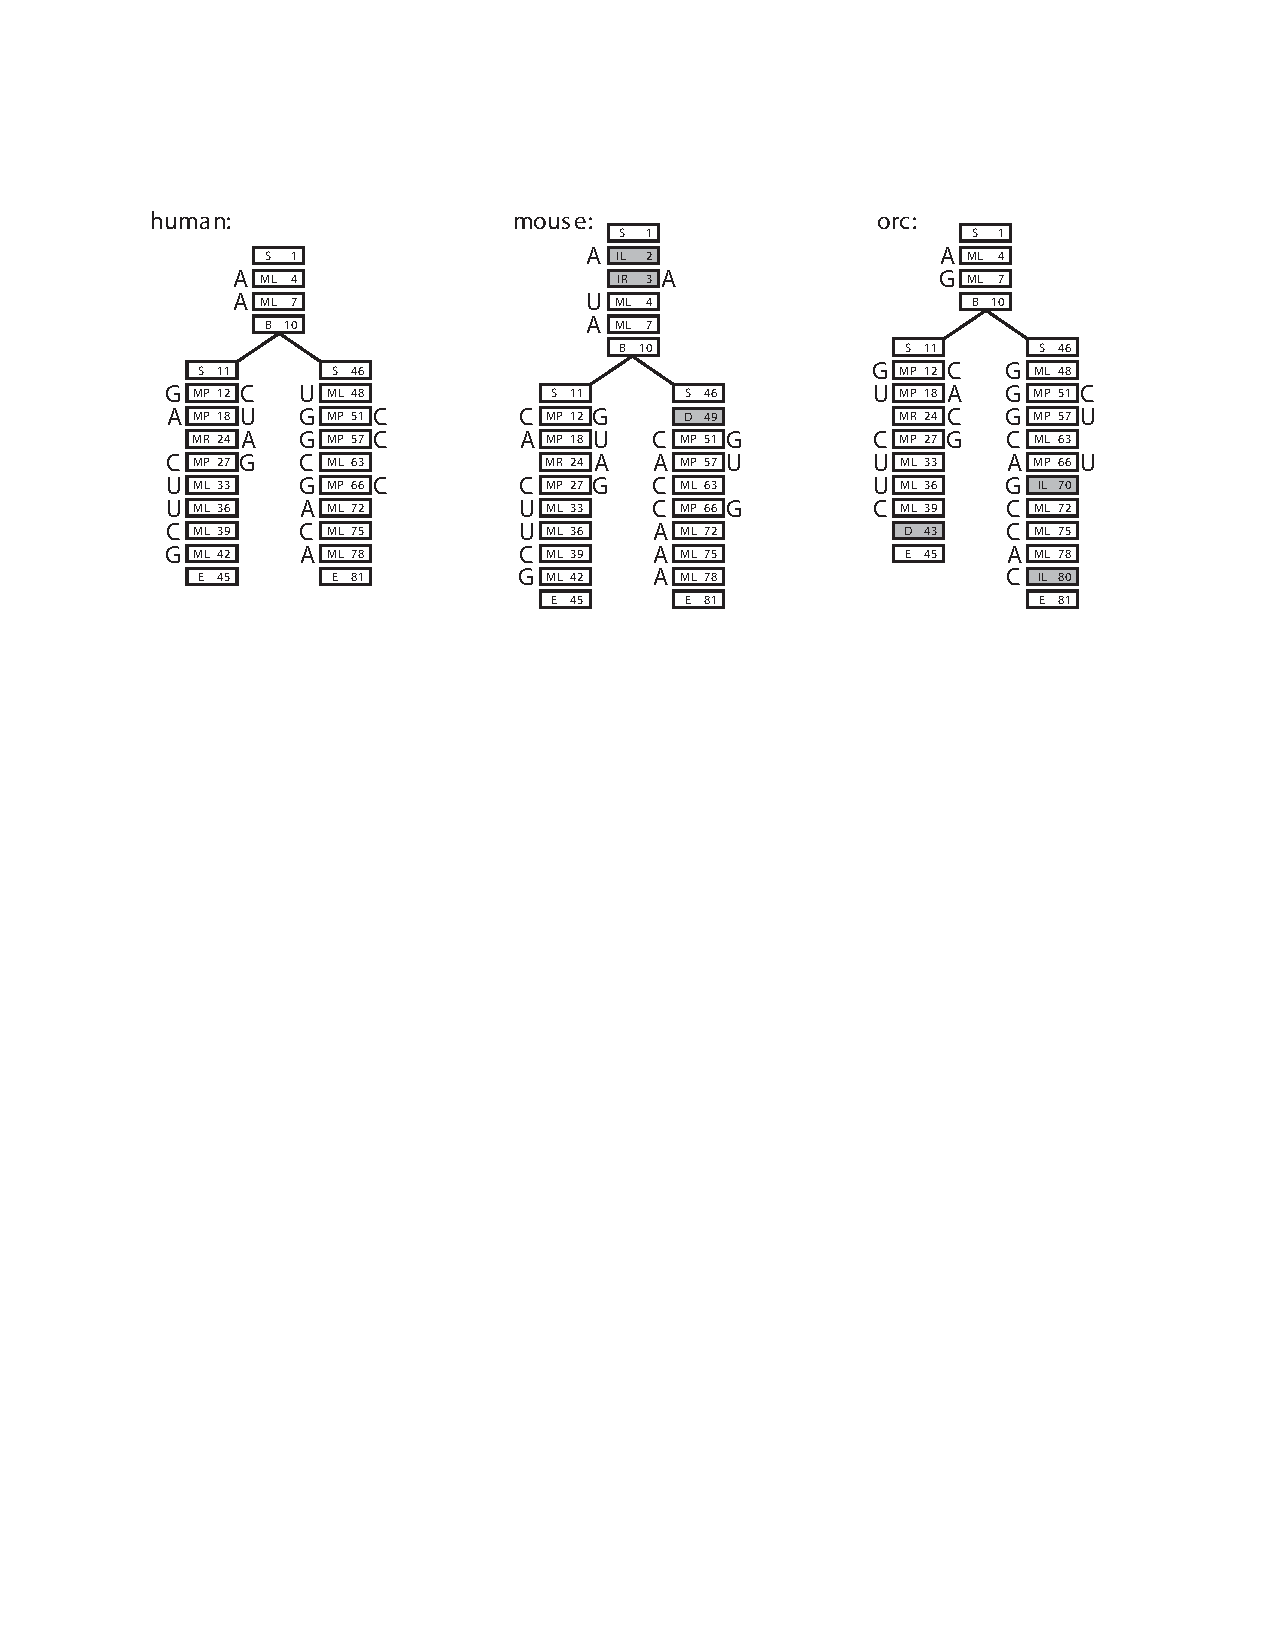
\includegraphics[width=5in]{Figures/parsetrees}
\end{center}
\caption{\textbf{Example parse trees.} Parse trees are shown for the
three sequences/structures from Figure~\ref{fig:input_alignment},
given the CM in Figure~\ref{fig:cm_graph}. For each sequence, each
residue must be associated with a state in the parse tree. (The
sequences can be read off its parse tree by starting at the upper left
and reading counterclockwise around the edge of parse tree.) Each
parse tree corresponds directly to a secondary structure -- base pairs
are pairs of residues aligned to MP states. A collection of parse
trees also corresponds to a multiple alignment, by aligning residues
that are associated with the same state -- for example, all three
trees have a residue aligned to state ML4, so these three residues
would be aligned together. Insertions and deletions relative to the
consensus use nonconsensus states, shown in gray.}
\label{fig:parsetrees}
\end{figure}
\fi

\subsubsection{Comparison to profile HMMs}

The relationship between an SCFG and a covariance model is analogous
to the relationship of hidden Markov models (HMMs) and profile HMMs
for modeling multiple sequence alignments
\cite{Krogh94,Durbin98,Eddy98}. A comparison may be instructive to
readers familiar with profile HMMs.  A profile HMM is a repetitive HMM
architecture that associates each consensus column of a multiple
alignment with a single type of model node -- a MATL node, in the
above notation. Each node contains a ``match'', ``delete'', and
``insert'' HMM state -- ML, IL, and D states, in the above notation.
The profile HMM also has special begin and end states. Profile HMMs
could therefore be thought of as a special case of CMs. An
unstructured RNA multiple alignment would be modeled by a guide tree
of all MATL nodes, and converted to an unbifurcated CM that would
essentially be identical to a profile HMM. (The only difference is
trivial; the CM root node includes a IR state, whereas the start node
of a profile HMM does not.) All the other node types (especially MATP,
MATR, and BIF) and state types (e.g. MP, MR, IR, and B) are SCFG
augmentations necessary to extend profile HMMs to deal with RNA
secondary structure.

The SCFG Inside and Outside algorithms are analogous to the Forward
and Backward algorithms for HMMs \cite{Rabiner89,Durbin98}.  The
CYK/inside parsing algorithm is analogous to the Viterbi HMM alignment
algorithm run in the forward direction. CYK/outside is analogous to a
Viterbi DP algorithm run in the backwards direction.


%%%%%%%%%%%%%%%%%%%%%%%%%%%%%%%%%%%%%%%%%%%%%%%%%%%%%%%%%%%%%%%%
%%%%%%%%%%%%%%%%%%%%%%%%%%%%%%%%%%%%%%%%%%%%%%%%%%%%%%%%%%%%%%%%

\subsection{Divide and conquer algorithm}

\subsubsection{Notation}

I use $r$, $v$, $w$, $y$, and $z$ as indices of states in the model,
where $r \leq (v,w,y) \leq z$. These indices will range from $1..M$, for
a CM with $M$ states. $G$. $G^r_z$ refers to a subgraph of the model,
rooted at state $r$ and ending at state $z$, for a contiguous set of
states $r..z$. $G^r$, without a subscript, refers to a subgraph of the
model rooted at state $r$ and ending at the highest numbered E state
descendant from state $r$. The complete model is $G^1_M$, or $G^1$, or
just $G$.

$S_v$ refers to the \emph{type} of state $v$; it will be one of seven
types \{D,P,L,R,S,E,B\}. $C_v$ is a list of children for state $v$
(e.g. the states that $v$ can transit to); it will contain up to six
contiguous indices $y$ with $v \leq y \leq M$. $P_v$ is a list of
parents for state $v$ (states that could have transited to state $v$);
it will contain up to six contiguous indices $y$ with $1 \leq y \leq
v$. ($P_v$ parent lists should not be confused with P state types.)

I use $g$, $h$, $i$, $j$, $k$, $p$, and $q$ as indices referring to
positions in a sequence $x$, where $g \leq h \leq p \leq q$ and $i
\leq j$ for all subsequences of nonzero length. These indices range
from $1..L$, for a sequence of length $L$. Some algorithms will also
use $d$ to refer to a subsequence length, where $d = j-i+1$ for a
subsequence $x_i..x_j$.

The algorithms will have to account for subsequences of zero length
(because of deletions). By convention, these will be in the
off-diagonal where $j = i-1$ or $i = j+1$. This special case (usually
an initialization condition) is the reason for the qualification that
$i \leq j$ for subsequences of \emph{nonzero} length.

The CYK/inside algorithm calculates a three-dimensional matrix of
numbers $\alpha_v(i,j)$, and CYK/outside calculates numbers
$\beta_v(i,j)$. I will refer to $v$ (state indices) as \emph{deck}
coordinates in the three-dimensional matrices, whereas $j$ and $i$
(sequence positions) are row and column coordinates within each deck.
$\alpha_{v}$ and $\beta_{v}$ refer to whole two-dimensional decks
containing scores $\alpha_v(i,j)$ and $\beta_v(i,j)$ for a particular
state $v$. The dividing and conquering will be done in the $v$
dimension, by choosing particular decks as split points.

\subsubsection{The CYK/inside algorithm}

The CYK/inside algorithm iteratively calculates $\alpha_v(i,j)$ -- the
log probability of the most likely CM parse subtree rooted at state
$v$ that generates subsequence $x_i..x_j$ of sequence $x$. The
calculation initializes at the smallest subgraphs and subsequences
(e.g. subgraphs rooted at E states, generating subsequences of length
0), and iterates outwards to progessively longer subsequences and
larger CM subgraphs.

For example, if we're calculating $\alpha_v(i,j)$ and $S_v =$ P (that
is, $v$ is a pair state), $v$ will generate the pair $x_i,x_j$ and
transit to a new state $y$ (one of its possible transitions $C_v$)
which then will have to account for the smaller subsequence
$x_{i+1}..x_{j-1}$. The log probability for a particular choice of
next state $y$ is the sum of three terms: an emission term $\log
e_v(x_i,x_j)$, a transition term $\log t_v(y)$, and an already
calculated solution for the smaller optimal parse tree rooted at $y$,
$\alpha_y(i+1,j-1)$. The answer for $\alpha_v(i,j)$ is the maximum
over all possible choices of child states $y$ that $v$ can transit to.

The algorithm \texttt{inside} is as follows:

\begin{algorithm}
\alginout{A CM subgraph $G^r_z$ and subsequence $x_g..x_q$.}
         {Scoring matrix decks $\alpha_r..\alpha_z$.}
\algname{inside}{r,z; g,q} 
\begin{algtab*}
\algforto{$v \leftarrow z$ \textbf{down}}{$r$}
  \algforto{$j \leftarrow g-1$}{$q$} 
    \algforto{$i \leftarrow j+1$ \textbf{down}}{$g$}
       $d \leftarrow j-i+1$\\
       \algif{$S_v =$ D or S:}
       	$\alpha_v(i,j) = \max\limits_{y \in C_v} \left[ \alpha_y(i,j)  + \log t_v(y) \right]$\\
       \algelseif{$S_v =$ P and $d \geq 2$:}
	$\alpha_v(i,j) = \log e_v(x_i, x_j) + \max\limits_{y \in C_v} \left[ \alpha_y(i+1,j-1) + \log t_v(y) \right]$\\
       \algelseif{$S_v =$ L and $d\geq1$:}
        $\alpha_v(i,j) = \log e_v(x_i) + \max\limits_{y \in C_v} \left[ \alpha_y(i+1,j)   + \log t_v(y) \right]$\\
       \algelseif{$S_v =$ R and $d\geq1$:}
        $\alpha_v(i,j) = \log e_v(x_j) +      \max\limits_{y \in C_v} \left[ \alpha_y(i,j-1)   + \log t_v(y) \right]$ \\
       \algelseif{$S_v =$ B:}
        $(y,z) \leftarrow $ left and right S children of state $v$\\
        $\alpha_v(i,j) = \max\limits_k \left[ \alpha_y(i,k) + \alpha_z(k+1,j) \right]$ \\
       \algelseif{$S_v =$ E and $d=0$:}
	$\alpha_v(i,j) = 0$  (initializations)\\
       \algelse
	$\alpha_v(i,j) = -\infty$ (initializations)\\
\end{algtab*}
\end{algorithm}

Given a sequence $x$ of length $L$ and a CM $G$ of length $M$, we
could call \texttt{inside(1,M; 1,L)} to align the whole model (states
$1..M$) to the whole sequence ($x_1..x_L$). When \texttt{inside}
returns, $\alpha_1(1,L)$ would contain the log probability of the best
parse of the complete sequence with the complete model. 

We do not have to keep the entire $\alpha$ three-dimensional matrix in
memory to calculate these scores.  As we reach higher decks $\alpha_v$
in the three dimensional dynamic programming matrix, our calculations
no longer depend on certain lower decks. A lower deck $y$ can be
deallocated whenever all the parent decks $P_y$ that depend on it
have been calculated. \footnote{The implementation goes even further
and recycles decks when possible, saving some initialization steps and
many memory allocation calls; for example, since values in all E decks
are identical, only one E deck needs to be calculated and that
precalculated deck can be reused whenever $S_v = E$.}

This deallocation rule has a important property that the divide and
conquer algorithm takes advantage of when solving smaller subproblems
for CM subgraphs rooted at some state $w$.  When the root state $w$ is
an S state, the $\alpha$ matrix returned by \texttt{inside} contains
only one active deck $\alpha_w$. (No lower state $>w$ can be reached
from any state $<w$ without going through $w$, so all lower decks are
deallocated once deck $w$ is completed.) When the root state $w$ is
the first state in a split set $w..y$ (see below for more
explanation), all (and only) the decks $\alpha_w..\alpha_y$ are active
when \texttt{inside} returns.

In some cases we want to recover the optimal parse tree itself, not
just its score. The \texttt{inside}$^{\mathcal{T}}$ routine is a
modified version of $\texttt{inside}$. It keeps an additional ``shadow
matrix'' $\tau_v(i,j)$. A $\tau_v(i,j)$ traceback pointer either
records the index $y$ that maximized $\alpha_v(i,j)$ (for state types
D,S,P,L,R) or records the split point $k$ that maximized
$\alpha_v(i,j)$ for a bifurcation (B) state. The $\tau$ shadow matrix
does not use the deallocation rules -- \texttt{inside}$^{\mathcal{T}}$
can only be called for problems small enough that they can be solved
within our available memory space. Thus the
\texttt{inside}$^{\mathcal{T}}$ routine works by calling
\texttt{inside} in a mode that also keeps a shadow matrix $\tau$,
and then calls a recursive traceback starting with $v,i,j$:

\begin{algorithm}
\alginout{A shadow matrix $\tau$ for CM subgraph $G^v$ rooted at state
         $v$, and subsequence $x_i..x_j$.}
         {An optimal parse tree $\mathcal{T}$.}
\algname{traceback}{v,i,j}
\begin{algtab*}
  \algif{$S_v =$ E:}
    attach $v$\\
  \algelseif{$S_v =$ S or D:}
    attach $v$ \\
    \algcall{traceback}{$\tau_v(i,j), i, j$}\\
  \algelseif{$S_v =$ P:}
    attach $x_i,v,x_j$\\
    \algcall{traceback}{$\tau_v(i,j), i+1, j-1$}\\
  \algelseif{$S_v =$ L:}
    attach $x_i,v$\\
    \algcall{traceback}{$\tau_v(i,j), i+1, j$}\\
  \algelseif{$S_v =$ R:}
    attach $v,x_j$\\
    \algcall{traceback}{$\tau_v(i,j), i,   j-1$}\\
  \algelseif{$S_v =$ B:}
    $(y,z) \leftarrow $ left and right S children of state $v$\\
    attach $v$\\
    \algcall{traceback}{$y, i, \tau_v(i,j)$}\\
    \algcall{traceback}{$z, \tau_v(i,j)+1, j$}\\
\algend
\end{algtab*}
\end{algorithm}

\subsubsection{The CYK/outside algorithm}

The CYK/outside algorithm iteratively calculates $\beta_v(i,j)$, the
log probability of the most likely CM parse tree for a CM generating a
sequence $x_1..x_L$ \emph{excluding} the optimal parse subtree rooted
at state $v$ that accounts for the subsequence $x_i..x_j$. The
calculation initializes with the entire sequence excluded (e.g.
$\beta_1(1,L) = 0$), and iterates inward to progressively shorter and
shorter excluded subsequences and smaller CM subgraphs.

A complete implementation of the CYK/outside algorithm requires first
calculating the CYK/inside matrix $\alpha$, because it is needed to
calculate $\beta_v$ when the parent of $v$ is a bifurcation
\cite{Lari90,Lari91,Durbin98}. However, the divide and conquer
algorithm described here only calls \texttt{outside} on
\emph{unbifurcated, linear CM subgraphs}; the parent of $v$ is never a
bifurcation, and the implementation can therefore be streamlined as
follows:

\begin{algorithm}
\alginout{An unbifurcated CM subgraph $G^r_z$ and subsequence $x_g..x_q$.}
         {Scoring matrix decks $\beta_r..\beta_z$.}
\algname{outside}{r,z; g,q}
\begin{algtab*}
 $\beta_v(i,j) \leftarrow -\infty \quad \forall \quad v,i,j$\\
 $\beta_r(g,q) \leftarrow 0$\\
 \algforto{$v \leftarrow r+1$}{$z$}
   \algforto{$j \leftarrow q$ \textbf{down}}{$g-1$}
     \algforto{$i \leftarrow g$}{$j+1$}
       $\beta_v(i,j) = \max\limits_{y \in P_v} \left\{
              \begin{array}{rcl}
              \beta_y(i,j) + \log t_y(v) &:&  S_y = D,S,E \\
              \beta_y(i-1,j+1) + \log t_y(v) + \log e_y(x_{i-1}, x_{j+1}) &:& S_y = P\\
              \beta_y(i-1,j) + \log t_y(v) + \log e_y(x_{i-1}) &:& S_y = L\\
              \beta_y(i,j+1) + \log t_y(v) + \log e_y(x_{j+1})  &:& S_y = R \\
              \end{array} \right.$
\end{algtab*}
\end{algorithm}

As with \texttt{inside}, we do not keep the entire $\beta$ matrix in
memory. A deck $\beta_v$ can be deallocated when all child decks $C_v$
that depend on the values in $\beta_v$ have been calculated. This
means that if the last deck $z$ is a bifurcation or end state,
$\beta_z$ will be the only active allocated deck when \texttt{outside}
returns. If $z$ is the last state in a split set $w..z$, all (and
only) the split set decks $\beta_w..\beta_z$ will be active when
\texttt{outside} returns.

\subsubsection{Using CYK/inside and CYK/outside to divide and conquer}

Now, for any chosen state $v$, $\argmax\nolimits_{i,j} \left[ \alpha_{v}(i,j) +
\beta_{v}(i,j) \right]$ tells us which cell $v,i,j$ the optimal parse tree
passes through, conditional on using state $v$ in the parse. We know
that any parse tree must include all the bifurcation and start states
of the CM, so we know that the optimal alignment \emph{must} use any
chosen bifurcation state $v$ and its child start states $w$ and
$y$. Thus, we are guaranteed that (when $S_v =$ B and $C_v = {w,y}$):
\[
   \max_{i,k,j} \left[ \beta_{v}(i,j) + \alpha_{w}(i,k) +
                       \alpha_{y}(k+1,j) \right]
\]
is the optimal overall alignment score, and we also know that
\[
      (i,k,j) = \argmax_{i',k',j'} \left[ \beta_{v}(i',j') +
      \alpha_{w}(i',k') + \alpha_{y}(k'+1,j')  \right]
\]
gives us a triplet that identifies three cells that must be in the
optimal alignment -- $(v,i,j)$, $(w,i,k)$, and $(y,k+1,j)$. This
splits the remaining problem into three smaller subproblems -- an
alignment of the sequence $x_{i}..x_{k}$ to a CM subgraph $w..y-1$, an
alignment of the sequence $x_{k+1}..x_{j}$ to a CM subgraph $y..M$,
and an alignment of the two-piece sequence
$x_1..x_{i-1}//x_{j+1}..x_L$ to a CM subgraph $1..v$.

The subproblems are then themselves split, and this splitting can
continue recursively until all the bifurcation triplets on the optimal
parse tree have been determined.

At this point the remaining alignment subproblems might be small
enough to be solved by straightforward application of the standard
CYK/inside algorithm (e.g. \texttt{inside}$^\mathcal{T}$). However,
this is not guaranteed to be the case. A more general division
strategy is needed that does not depend on splitting at bifurcations.

For the more general strategy we take advantage of the fact that we
know that the optimal parse tree must also include one and only one
state from the split set of each node (e.g. the non-insert states in
the node). Let $w..y$ be the indices of a split set of states in the
middle of the current model subgraph. ($w..y$ can be at most 4
states.)  We know that
\[
(v,i,j) = \argmax_{v' \in w..y,i',j'} \left[ \alpha_{v'}(i',j') +
\beta_{v'}(i',j') \right]
\]
gives us a new cell $(v,i,j)$ in the optimal parse tree, and splits
the problem into two smaller problems. This strategy can be applied
recursively all the way down to single nodes, if necessary. We can
therefore guarantee that we will never need to carry out a full
CYK/inside alignment algorithm on any subproblem. The most
memory-intensive alignment problem that needs to be solved is the very
first split.  The properties of the first split determine the memory
complexity of the algorithm.

The bifurcation-dependent strategy is a special case of this more
general splitting strategy, where the B state is the only member of
its split set, and where we also take advantage of the fact that
$\alpha_v(i,j) = \max_k \alpha_w(i,k) + \alpha_y(k+1,j)$. By carrying
out the $\max_k$ operation during the split, rather than before, we
can split the current problem into three optimal pieces instead of
just two.

If we look at the consequences of these splitting strategies, we see
we will have to deal with three types of problems
(Figure~\ref{fig:splitter_schematic}):

\begin{itemize}
\item A \emph{generic problem} means finding the optimal alignment of
a CM subgraph $G^r_z$ to a contiguous subsequence $x_g..x_q$. The
subgraph $G^r_z$ corresponds to a complete subtree of the CM's
guide tree -- e.g. state $r$ is a start (S), and state $z$ is an end
(E). $G^r_z$ may contain bifurcations. The problem is solved in one
of two ways. If $G^r_z$ contains no bifurcations, it is solved as a
wedge problem (see below). Else, the problem is subdivided by the
bifurcation-dependent strategy: an optimal triple $(i,k,j)$ is found
for a bifurcation state $v$ and its children $w,y$, splitting the
problem into a V problem and two generic problems.

\item A \emph{wedge problem} means finding the optimal alignment of an
\emph{unbifurcated} CM subgraph $G^r_z$ to a contiguous subsequence
$x_g..x_q$. State $r$ does not have to be a start state (S); it may be
a state in a split set (MP, ML, MR, or D). State $z$ is an end (E).  A
wedge problem is solved by the split set-dependent strategy: an
optimal $(v,i,j)$ is found, splitting the problem into a V problem and
a smaller wedge problem.

\item A \emph{V problem} consists of finding the optimal alignment of
an \emph{unbifurcated} CM subgraph $G^r_z$ to a noncontiguous,
two-piece sequence $x_g..x_h//x_p..x_q$, exclusive of the residues
$x_h$ and $x_p$ (open circles in Figure~\ref{fig:splitter_schematic}).
State $r$ can be a start state or any state in a split set; the same
is true for $z$. A V problem is solved by a split set-dependent
strategy: an optimal $(v,i,j)$ is found, splitting the problem into
two V problems.
\end{itemize}

\ifdraft
\begin{figure}
\begin{center}
\includegraphics[width=5in]{Figures/splitter_schematic}
\end{center}
\caption{\textbf{The three types of problems that need to be split.}
The sequence axis (e.g. $x_g..x_q$) is horizontal. The model subgraph
axis for a contiguous set of states (e.g. states $r..z$) is vertical,
where a solid lines means an unbifurcated model subgraph, and a dashed
line means a model subgraph that may contain bifurcations.  Closed
circles indicate ``inclusive of'', and open circles indicate
``exclusive of''.}
\label{fig:splitter_schematic}
\end{figure}
\fi

The three recursive splitting algorithms to solve these problems
are as follows:

\subsubsection{The generic\_splitter routine}
\begin{algorithm}
\alginout{A generic problem, for CM subgraph $G^r_z$ and
          subsequence $x_{g..q}$.}
         {An optimal parse subtree $\mathcal{T}$.}

\algname{generic\_splitter}{r,z; g,q}
\begin{algtab*}
\algif{no bifurcation in $G^r_z$:}
  \algreturn \algcall{wedge\_splitter}{r,z; g,q}\\
\algelse
   $v   \leftarrow$ lowest numbered bifurcation state in subgraph $G^r_z$.\\
   $w,y \leftarrow$ left and right S children of $v$.\\
   $\beta_v \leftarrow$  \algcall{outside}{r,w; g,q}\\
   $\alpha_w \leftarrow$ \algcall{inside}{w,y-1; g,q}\\
   $\alpha_y \leftarrow$ \algcall{inside}{y,z; g,q}\\

   $(i,k,j) \leftarrow \argmax_{i',k',j'} \left[ \alpha_w(i',k') +
   \alpha_y(k'+1,j') + \beta_v(i',j') \right] $ \\

   $\mathcal{T}_1   \leftarrow$ \algcall{V\_splitter}{r,v; g,i; j,q}\\
   $\mathcal{T}_2 \leftarrow$ \algcall{generic\_splitter}{w,y-1; i,k}\\
   $\mathcal{T}_3 \leftarrow$ \algcall{generic\_splitter}{y,z; k+1,j}\\

   Attach S state $w$ of $\mathcal{T}_2$ as left child of B state $v$ in $\mathcal{T}_1$.\\
   Attach S state $y$ of $\mathcal{T}_3$ as right child of B state $v$ in $\mathcal{T}_2$.\\
  
   \algreturn $\mathcal{T}_1$.\\
\algend
\end{algtab*}
\end{algorithm}

\subsubsection{The wedge\_splitter routine}
\begin{algorithm}
\alginout{A wedge problem, for unbifurcated CM subgraph $G^r_z$ and
          subsequence $x_{g..q}$.}
         {An optimal parse subtree $\mathcal{T}$.}

\algname{wedge\_splitter}{r,z; g,q}
\begin{algtab*}
  $(w..y) \leftarrow$ a split set chosen from middle of $G^r_z$\\
  $(\alpha_w..\alpha_y) \leftarrow$ \algcall{inside}{w,z; g,q}\\
  $(\beta_w..\beta_y)   \leftarrow$ \algcall{outside}{r,y; g,q}\\
  $(v,i,j) \leftarrow \argmax\limits_{v',i',j'}  \left[
	\alpha_{v'}(i',j') + \beta_{v'}(i',j') \right]$\\
  $\mathcal{T}_1 \leftarrow$ \algcall{V\_splitter}{r,v; g,i; j,q}\\
  $\mathcal{T}_2 \leftarrow$ \algcall{wedge\_splitter}{v,z; i,j}\\
  Attach $\mathcal{T}_2$ to $\mathcal{T}_1$ by merging at state $v$.\\
  
  \algreturn $\mathcal{T}_1$.\\
\algend
\end{algtab*}
\end{algorithm}

\subsubsection{The V\_splitter routine}
\begin{algorithm}
\alginout{A V problem, for unbifurcated CM subgraph $G^r_z$ and
          two-part subsequence $x_{g..h}//x_{p..q}$.}
         {An optimal parse subtree $\mathcal{T}$.}

\algname{V\_splitter}{r,z; g,h; p,q}
\begin{algtab*}
  $(w..y) \leftarrow$ a split set chosen from middle of $G^r_z$\\
  $(\alpha_w..\alpha_y) \leftarrow$ \algcall{vinside}{w,z; g,h; p,q}\\
  $(\beta_w..\beta_y)   \leftarrow$ \algcall{voutside}{r,y; g,h; p,q}\\
  $(v,i,j) \leftarrow \argmax_{v'=w..y, i'=g..h, j'=p..q}  \left[
	\alpha_{v'}(i',j') + \beta_{v'}(i',j') \right]$ \\
  $\mathcal{T}_1 \leftarrow$ \algcall{V\_splitter}{r,v; g,i; j,q}\\
  $\mathcal{T}_2 \leftarrow$ \algcall{V\_splitter}{v,z; i,h; p,j}\\
  Attach $\mathcal{T}_2$ to $\mathcal{T}_1$ by merging at state $v$.\\
  \algreturn $\mathcal{T}_1$.\\
\algend
\end{algtab*}
\end{algorithm}

\subsubsection{The vinside and voutside routines}

The \texttt{vinside} and \texttt{voutside} routines are just
\texttt{inside} and \texttt{outside}, modified to deal with a
two-piece subsequence $x_g..x_h//x_p..x_q$ instead of a contiguous
sequence $x_g..x_q$. These modifications are fairly obvious. The
range of $i,j$ is restricted so that $i \leq h$ and $j \geq p$.  Also,
\texttt{vinside(w,z; g,h; p,q)} initializes $\alpha_z(h,p) = 0$: that
is, we know that sequence $x_h..x_p$ has already been accounted for by
a CM parse tree rooted at $z$.

\subsubsection{Implementation}

In the description of the algorithms above, some technical detail has
been omitted - in particular, a detailed description of efficient
initialization steps, and details of how the the dynamic programming
matrices are laid out in memory. These details are not necessary for a
high level understanding of the divide and conquer algorithm. However,
they may be necessary for reproducing a working
implementation. Commented ANSI/C source code for a reference
implementation is therefore freely available at
\url{http://www.genetics.wustl.edu/eddy/infernal/} under a GNU General
Public License. This code has been tested on GNU/Linux platforms.

In this codebase, the CM data structure is defined in
\texttt{structs.h}. The CM construction procedure is in
\texttt{modelmaker.c:Handmodelmaker()}. The guide tree is constructed
in \texttt{HandModelmaker()}. A CM is constructed from the guide tree
by \texttt{cm\_from\_master()}. Individual parse trees are constructed
using the guide tree by \texttt{transmogrify()}.  The divide and
conquer algorithm is implemented in
\texttt{smallcyk.c:CYKDivideAndConquer()}, which will recursively call
a set of functions: the three splitting routines
\texttt{generic\_splitter()}, \texttt{wedge\_splitter()}, and
\texttt{v\_splitter()}; the four alignment engines \texttt{inside()},
\texttt{outside()}, \texttt{vinside()}, and \texttt{voutside()}; and
the two traceback routines \texttt{insideT()} and \texttt{vinsideT()}.


%%%%%%%%%%%%%%%%%%%%%%%%%%%%%%%%%%%%%%%%%%%%%%%%%%%%%%%%%%%%%%%%
%%%%%%%%%%%%%%%%%%%%%%%%%%%%%%%%%%%%%%%%%%%%%%%%%%%%%%%%%%%%%%%%

\section{Results and discussion}

\subsection{Memory complexity analysis}

The memory complexity of normal CYK/inside is $O(N^2M)$, for a model
of $M$ states and a query sequence of $N$ residues, since the full 3D
dynamic programming matrix is indexed $N \times N \times M$ (and since
$N \propto M$, we can alternatively state the upper bound as
$O(N^3)$). The memory complexity of the divide and conquer algorithm
is $O(N^2 \log M)$. The analysis that leads to this conclusion is as
follows.

For a model with no bifurcations, the divide and conquer algorithm
will never require more than 10 decks in memory at once. In the case
of two adjacent MATP nodes, we will need six decks to store the scores
for the current node we're calculating, and four decks for the split
set of the adjacent node that we're connecting to (and dependent
upon) (Figure~\ref{fig:cm_graph}).

Bifurcations will require some number of additional decks for start
states (BEGL\_S and BEGR\_S) to be kept. In \texttt{inside}, whenever
we reach a deck for a start state, we will keep that deck in memory
until we reach the parent bifurcation state. Half the time, that will
mean waiting until another complete subgraph of the model is
calculated (e.g. the subgraph rooted at the other start child of that
bifurcation); that is, to calculate deck $\alpha_v$ for a bifurcation
$v$, we need both decks $\alpha_w$ and $\alpha_y$ for its child start
states $w$ and $y$, so we have to hold on to $\alpha_y$ until we reach
$\alpha_w$. In turn, the subgraph rooted at $w$ might contain
bifurcations, so our calculation of $\alpha_w$ might require
additional decks to be kept. Each start deck we reach in the
\texttt{inside} iteration means holding one extra deck in memory, and
each bifurcation we reach means deallocating the two start decks it
depends on; therefore we can iteratively calculate the maximum number
of extra decks we will require:

\begin{algorithm}
\begin{algtab*}
  $x_M \leftarrow -1$\\
  \algforto{$v \leftarrow M-1$}{1}
     $x_v \leftarrow \left\{ 
       \begin{array}{rcl} 
        x_{v+1} + 1 &:& S_v = S,\\
        x_{v+1} - 2 &:& S_v = B,\\
        x_{v+1}     &:& \mbox{elsewise.}\\
       \end{array} \right.$\\
  \algreturn{$\max_v x_v$}\\
\end{algtab*}
\end{algorithm}

This number depends on the topology and order of evaluation of the
states in the CM. Think of the bifurcating structure of the CM as a
binary tree numbered in preorder traversal (e.g. left children are
visited first, and have lower indices than right children). If this is
a complete balanced tree with $B$ bifurcations, we will need $\log_2
B$ extra decks. If it is a maximally unbalanced tree in which
bifurcations only occur in left children, we will need $B$ extra decks
(all the right children). If it is a maximally unbalanced tree in
which bifurcations only occur in right children, we will only ever
need 1 extra deck. A left-unbalanced binary tree can be converted to a
right-unbalanced binary tree just by swapping branches. For a CM, we
can't swap branches without affecting the order of the sequence that's
generated. We can, however, get the same effect by renumbering the CM
states in a modified preorder traversal. Instead of always visiting
the left subtree first, we visit the best subtree first, where
``best'' means the choice that will optimize memory usage.  This
reordering is readily calculated in $O(M)$ time (not shown; see
\texttt{cm.c:CMRebalance()} in the implementation).  This way, we can
never do worse than the balanced case, and we will often do better. We
never need more than $\log_2 B$ extra decks. Since $B < M$, we can
guarantee a $O(N^2 \log M)$ bound on memory complexity.

\subsection{Time complexity analysis}

The time complexity of the standard algorithm is $O(MN^2 + BN^3)$, for
a model of $M$ states ($B$ of which are bifurcations) aligned to a
sequence of $N$ residues. Since $B < M$, and $M \propto N$, we can
also state the upper bound as $O(MN^3)$ or $O(N^4)$.

The time complexity of the divide and conquer algorithm depends on how
close each split is to dividing a problem into equal sized
subproblems. In the most ideal case, each call to
\texttt{generic\_splitter} could split into three subproblems that
each contained $1/3$ of the states and residues: splitting those three
subproblems would only cost $3 \times (\frac{1}{3})^4 \times MN^3$ in
time, e.g. only about $1/27$ the time it took to split the first
problem. Thus in an ideal case the time requirement is almost
completely dominated by the first split, and the extra time required
to do the complete divide and conquer algorithm could be
negligible. In pathological cases, optimal splits might lead to a
series of very unequally sized problems. We never need to do more splits
than there are states in the model, so we cannot do worse than
$O(M^2N^3)$ in time.

An example of a pathological case is an RNA structure composed of a
series of multifurcation loops such that each bifurcation leads to a
small stem on one side, and the rest of the structure on the other. In
such a case, every call to \texttt{generic\_splitter()} will split
into a small subproblem containing a small stem (e.g. only removing a
constant number of states and residues per split) and a large
subproblem containing all the remaining states and sequence. This case
can be avoided. It only arises because of the decision to implement a
simplified CYK/outside algorithm and always split at the highest
bifurcations. Better time performance could be guaranteed if a
complete CYK/outside algorithm were implemented (at the cost of
complexity in the description and implementation of the algorithm).
This would allow us to choose a split point in a generic problem at
any state in the CM (for instance, in the middle) regardless of its
bifurcating structure.

In practice, empirical results on a variety of real RNAs (see below)
indicate that the extra time required to do the divide and conquer is
a small constant factor. A more complex implementation does not seem
to be necessary.

\subsection{Empirical results}

Six structural RNA families were chosen for empirical evaluations of
the algorithm, using available RNA database resources -- tRNA
\cite{Steinberg93}, 5S ribosomal RNA \cite{Szymanski02}, signal
recognition particle (SRP) RNA \cite{Larsen91}, RNase P
\cite{Brown99}, small subunit (SSU) ribosomal RNA \cite{Neefs93}, and
large subunit (LSU) ribosomal RNA \cite{deRijk94}. For each family, a
secondary structure annotated multiple alignment of four or five
example sequences was extracted, and used to construct a CM. 

The top of Table~\ref{tbl:results} shows some statistics about these
alignments and CMs. The number of consensus columns in the alignments
ranges from 72 (tRNA) to 2898 (LSU rRNA); about 55-60\% are involved
in consensus base pairs. The number of CM states is consistently about
3-fold more than the consensus alignment length, ranging from 230
states (tRNA) to 9023 (LSU). About 1/150 of the states in each model
are bifurcations. After optimal reordering of the model states, the
number of extra decks required by the alignment algorithm is small,
ranging up to 3 for SSU and 5 for LSU rRNA. Therefore the minimum
constant of 10 decks required in iterations across unbifurcated model
segments dominates the memory requirement. The memory required for
extra decks does not have much impact even for the largest structural
RNAs. (Even without optimal reordering, the number of extra decks
required for SSU and LSU are only 7 and 9, respectively. State
reordering was only needed to assure a $O(N^2\log M)$ memory
complexity bound.)

To determine the memory and CPU time requirements for a structural
alignment, one example sequence from each family was aligned to the
CM. CPU time was measured and memory requirements were calculated for
three algorithms: (1) the full CYK/inside algorithm, but in
memory-saving score-only mode (e.g. \texttt{inside(1,M; 1,L}); (2) the
full CYK/inside algorithm, with shadow matrix and traceback to recover
the optimal alignment (e.g. \texttt{inside}$^\mathcal{T}$\texttt{(1,M;
1,L))}; and (3) the divide and conquer algorithm to recover an optimal
alignment (e.g. \texttt{generic\_splitter(1,M; 1,L)}). The most
important comparison is between the full CYK/inside algorithm and the
divide and conquer algorithm. The score-only CYK/inside algorithm was
included, because a complete CYK alignment couldn't be done on SSU and
LSU rRNA (because of the steep memory requirement). In all cases where
comparison could be done, the scores and alignments produced by these
algorithms were verified to be identical.

\ifdraft
\begin{table}
\begin{tabular}{lrrrrrr} 
                             & tRNA&5S rRNA& SRP RNA&RNase P& SSU rRNA& LSU rRNA \\\hline
\# of consensus columns      &  72 &  116 &   301 &   379 &   1545 &    2898\\ 
\# of consensus base pairs   &  21 &   35 &    89 &   113 &    462 &     794\\ 
\# of consensus unpaired     &  30 &   46 &   123 &   153 &    621 &    1310\\ 
CM states ($M$)              & 230 &  357 &   927 &  1176 &   4789 &    9023\\ 
bifurcations ($B$)           &   2 &    1 &     4 &     7 &     30 &      65\\ 
Maximum extra decks needed   &   1 &    1 &     2 &     2 &      3 &       5\\ 
Example sequence length ($N$)&  73 &  120 &   300 &   377 &   1542 &    2904\\
Full CYK RAM (MB)            & 2.6 & 10.7 & 168.9 & 336.7 &22705.0 &151349.7\\
Divide \& conquer RAM (MB)   & 0.1 &  0.4 &   2.4 &   3.7 &   66.8 &   270.9\\ 
Full CYK CPU time (sec)      & 0.2 &  0.7 &  12.7 &  28.6 &   n.d. &    n.d.\\ 
CYK CPU time, no trace (sec) & 0.1 &  0.6 &  10.4 &  23.8 & 2614.8 & 25151.2\\
Divide \& conquer time (sec) & 0.2 &  0.9 &  22.8 &  37.8 & 3594.4 & 31649.4\\\hline
\end{tabular}
\caption{Results of empirical tests of memory and CPU time required by
CM structural alignment algorithms on six known structural RNAs of
various sizes.}
\label{tbl:results}
\end{table}
\fi

The results of these tests are shown in the bottom half of
Table~\ref{tbl:results}. The memory required by divide and conquer
alignment ranges up to 271 MB for LSU rRNA, compared to a prohibitive
151 GB for the standard CYK algorithm. The extra CPU time required by
the divide and conquer is small; usually about 20\% more, with a
maximum of about two-fold more for SRP-RNA.

\ifdraft
\begin{figure}[ht]
\begin{center}
\includegraphics[width=5.5in]{Figures/graphs}
\end{center}
\caption{\textbf{Empirical time and memory requirements for structural
alignment.} Plots of data from Table~\ref{tbl:results}. Filled
circles: divide and conquer algorithm; open circles: standard CYK
algorithm. Left: Memory use in megabytes on a log-log scale. Lines
represent weighted least-squares regression fits to the theoretically
expected memory scaling: $aN^2 \log N$ for divide and conquer (solid
line) and $aN^3$ for standard CYK (dashed line). Right: CPU times in
seconds on a log-log scale. Lines represent least-squares regression
fits to a power law ($aN^b$).  According to this fit, divide and
conquer time (solid line) empirically scales as $N^{3.24}$, and
standard CYK without traceback (dashed line) scales as $N^{3.29}$. A
line representing $O(N^4)$ scaling (the theoretical upper bound on
performance) is shown for comparison.}
\label{fig:graphs}
\end{figure}
\fi

The same results are plotted in Figure~\ref{fig:graphs}. Memory
requirements scale as expected: $N^3$ for standard CYK alignment, and
better than $N^2 \log N$ for the divide and conquer algorithm.
Empirical CPU time requirements scale similarly for the two algorithms
$(N^{3.24}-N^{3.29})$. The observed performance is better than the
theoretical worst case of $O(N^4)$. The proportion of extra time
required by divide and conquer is roughly constant over a wide range
of RNAs. The difference shown in Figure~\ref{fig:graphs} is
exaggerated because times are plotted for score-only CYK, not complete
CYK alignment, in order to include CPU times for SSU and LSU
rRNA. Because score-only CYK does not keep a shadow traceback matrix
nor perform the traceback, it is about 20\% faster than CYK alignment,
as seen in the data in Table~\ref{tbl:results}.

\section{Conclusions}

The divide and conquer algorithm described here makes it possible to
align even the largest structural RNAs to secondary structure
consensus models, without exceeding the available memory on current
computational hardware. Optimal SSU and LSU rRNA structural alignments
can be performed in 70 MB and 270 MB of memory, respectively. Previous
structural alignment algorithms had to sacrifice mathematical
optimality to achieve ribosomal RNA alignments.

The CPU time requirement of the alignment algorithm is still
significant, and even prohibitive for certain important
applications. However, CPU time is generally an easier issue to deal
with. A variety of simple parallelization strategies are
possible. Banded dynamic programming algorithms (e.g. calculating only
relevant parts of the matrix) of various forms can also be explored,
including not only heuristic schemes, but also optimal algorithms
based on branch and bound ideas. (Properly implemented, banded DP
algorithms would also save additional memory.)

The current implementation of the algorithm is not biologically
useful. It is meant only a testbed for the algorithm. It outputs a raw
traceback structure and alignment score, not a standardly formatted
alignment file. Most importantly, the probability parameters for
models are calculated in a very quick and simple minded fashion, and
are far from being reasonable for producing robustly accurate
structural alignments. The next step along this line is to produce
good prior distributions for estimating better parameters, by
estimating mixture Dirichlet priors from known RNA structures
\cite{Sjolander96}.  At this stage it would not be meaningful to
compare the biological alignment accuracy of this implementation to
(for instance) the excellent performance of the RAGA genetic algorithm
\cite{Notredame97}.  A biologically useful implementation with
accurate alignment performance is of course the eventual goal of this
line of work, but is not the point of the present paper.

\section{Acknowledgements}

I gratefully acknowledge financial support from the Howard Hughes
Medical Institute, NIH R01 HG01363, and Alvin Goldfarb. I also wish to
thank Elena Rivas and Robin Dowell for critical comments on the
manuscript.

\newpage
\bibliography{distilled}

\ifdraft
 \relax
\else
\newpage
\begin{table}[h]
\begin{tabular}{lrrrrrr} 
                             & tRNA&5S rRNA& SRP RNA&RNase P& SSU rRNA& LSU rRNA \\\hline
\# of consensus columns      &  72 &  116 &   301 &   379 &   1545 &    2898\\ 
\# of consensus base pairs   &  21 &   35 &    89 &   113 &    462 &     794\\ 
\# of consensus unpaired     &  30 &   46 &   123 &   153 &    621 &    1310\\ 
CM states ($M$)              & 230 &  357 &   927 &  1176 &   4789 &    9023\\ 
bifurcations ($B$)           &   2 &    1 &     4 &     7 &     30 &      65\\ 
Maximum extra decks needed   &   1 &    1 &     2 &     2 &      3 &       5\\ 
Example sequence length ($N$)&  73 &  120 &   300 &   377 &   1542 &    2904\\
Full CYK RAM (MB)            & 2.6 & 10.7 & 168.9 & 336.7 &22705.0 &151349.7\\
Divide \& conquer RAM (MB)   & 0.1 &  0.4 &   2.4 &   3.7 &   66.8 &   270.9\\ 
Full CYK CPU time (sec)      & 0.2 &  0.7 &  12.7 &  28.6 &   n.d. &    n.d.\\ 
CYK CPU time, no trace (sec) & 0.1 &  0.6 &  10.4 &  23.8 & 2614.8 & 25151.2\\
Divide \& conquer time (sec) & 0.2 &  0.9 &  22.8 &  37.8 & 3594.4 & 31649.4\\\hline
\end{tabular}
\caption{Results of empirical tests of memory and CPU time required by
CM structural alignment algorithms on six known structural RNAs of
various sizes.}
\label{tbl:results}
\end{table}

\newpage
\begin{figure}[h]
\caption{\textbf{An example RNA sequence family.} Top: a toy multiple
alignment of three sequences, with 28 total columns, 24 of which will
be modeled as consensus positions. The [structure] line annotates the
consensus secondary structure: $>$ and $<$ symbols mark base pairs,
x's mark consensus single stranded positions, and .'s mark
``insert'' columns that will not be considered part of the consensus
model. Bottom: the secondary structure of the ``human'' sequence.} 
\label{fig:input_alignment}
\end{figure}

\begin{figure}[h]
\caption{\textbf{The structural alignment is converted to a guide
tree.} Left: the consensus secondary structure is derived from the
annotated alignment in Figure~\ref{fig:input_alignment}. Numbers in
the circles indicate alignment column coordinates: e.g.  column 4 base
pairs with column 14, and so on. Right: the CM guide tree
corresponding to this consensus structure. The nodes of the tree are
numbered 1..24 in preorder traversal (see text). MATP, MATL, and MATR
nodes are associated with the columns they generate: e.g., node 6 is a
MATP (pair) node that is associated with the base-paired columns 4 and
14.}
\label{fig:cm_nodetree}
\end{figure}

\begin{figure}[h]
\caption{\textbf{A complete covariance model.} Right: the CM
corresponding to the alignment in Figure~\ref{fig:input_alignment}.
The model has 81 states (boxes, stacked in a vertical array). Each
state is associated with one of the 24 nodes of the guide tree (text
to the right of the state array). States corresponding to the
consensus are in white. States responsible for insertions and
deletions are gray. The transitions from bifurcation state B10 to
start states S11 and S46 are in bold because they are special: they
are an obligate (probability 1) bifurcation. All other transitions
(thin arrows) are associated with transition probabilities.  Emission
probability distributions are not represented in the figure. Left: the
states are also arranged according to the guide tree. A blow up of
part of the model corresponding to nodes 6, 7, and 8 shows
more clearly the logic of the connectivity of transition probabilities
(see main text), and also shows why any parse tree must transit through
one and only one state in each ``split set''.}
\label{fig:cm_graph}
\end{figure}

\begin{figure}[h]
\caption{\textbf{Example parse trees.} Parse trees are shown for the
three sequences/structures from Figure~\ref{fig:input_alignment},
given the CM in Figure~\ref{fig:cm_graph}. For each sequence, each
residue must be associated with a state in the parse tree. (The
sequences can be read off its parse tree by starting at the upper left
and reading counterclockwise around the edge of parse tree.) Each
parse tree corresponds directly to a secondary structure -- base pairs
are pairs of residues aligned to MP states. A collection of parse
trees also corresponds to a multiple alignment, by aligning residues
that are associated with the same state -- for example, all three
trees have a residue aligned to state ML4, so these three residues
would be aligned together. Insertions and deletions relative to the
consensus use nonconsensus states, shown in gray.}
\label{fig:parsetrees}
\end{figure}

\begin{figure}[h]
\caption{\textbf{The three types of problems that need to be split.}
The sequence axis (e.g. $x_g..x_q$) is horizontal. The model subgraph
axis for a contiguous set of states (e.g. states $r..z$) is vertical,
where a solid lines means an unbifurcated model subgraph, and a dashed
line means a model subgraph that may contain bifurcations.  Closed
circles indicate ``inclusive of'', and open circles indicate
``exclusive of''.}
\label{fig:splitter_schematic}
\end{figure}

\begin{figure}[h]
\caption{\textbf{Empirical time and memory requirements for structural
alignment.} Plots of data from Table~\ref{tbl:results}. Filled
circles: divide and conquer algorithm; open circles: standard CYK
algorithm. Left: Memory use in megabytes on a log-log scale. Lines
represent weighted least-squares regression fits to the theoretically
expected memory scaling: $aN^2 \log N$ for divide and conquer (solid
line) and $aN^3$ for standard CYK (dashed line). Right: CPU times in
seconds on a log-log scale. Lines represent least-squares regression
fits to a power law ($aN^b$).  According to this fit, divide and
conquer time (solid line) empirically scales as $N^{3.24}$, and
standard CYK without traceback (dashed line) scales as $N^{3.29}$. A
line representing $O(N^4)$ scaling (the theoretical upper bound on
performance) is shown for comparison.}
\label{fig:graphs}
\end{figure}

\newpage



\fi



\end{document}



